\documentclass[12pt,oneside,openany,a4paper,%..... Layout
               afrikaans, english,%.............. Global language selection
               ]{memoir}

 \usepackage[PhD,%.......................... phd thesis
             wideblock,%........................ A5 type block (or a5block or wide)
            ]{usthesis}%.......................... US thesis style with memoir

%
% PLEASE read the USthesis documentation for the class options
% and how to set line and paragraph spacing
%

%==== Language setup ================================================
 \usepackage[latin1]{inputenc}%................... Recognizes ê, ë, etc
 \usepackage{babel}%.............................. Language setup

%==== Math setup ====================================================
 \usepackage{amsmath}%............................ Advanced math (before fonts)
 %\usepackage{amssymb}%............................ AMS Symbol fonts

%==== Font setup (default is Computer Modern) =======================
 \usepackage[T1]{fontenc}%........................ Type 1 fonts
 %\usepackage{fourier}
 \usepackage{textcomp}%........................... Additional text character
 \usepackage{bm}%................................. Bold math symbols (after fonts)

%==== Ref's, Bib's and Nomencl ======================================
 \usepackage{usnomencl}%.......................... List of symbols (in usthesis pack)
 \usepackage{usbib}%.............................. Bibliography    (in usthesis pack)
    \bibliographystyle{ussagus}
    \renewcommand\bibfont{\small}

    %% For usmeg-a, the bib is a list of references. If you
    %% are using usmeg-n comment out the following lines
    \addto{\captionsafrikaans}{\renewcommand{\bibname}{Lys van Verwysings}}
    \addto{\captionsenglish}{\renewcommand{\bibname}{Bibliography}}

%==== Graphics and Color ============================================
\usepackage{graphicx}%........................... Graphicx loaded in usthesis
\usepackage{color}%.............................. Color setup
\usepackage{eso-pic}%............................ Shipout commands for watermark
    \newcommand*{\WaterMark}[2][0.15\paperwidth]{%
        \AddToShipoutPicture*{\AtTextCenter{%
                \parbox[c]{0pt}{\makebox[0pt][c]{%
                    \includegraphics[width=#1]{#2}}}}}}

%==== Local Defs ====================================================
\makeatletter

%
% Please insert user defined commands here
% and NOT in the document itself!
%

\makeatother

%==== TITLE PAGE ====================================================
\title{\bfseries
       \AorE{%-- Afrikaans ------------------------------------------
             Diskrete Element Modellering van 'n Vibrerende Skeurploeg\\[1ex]
             \normalfont\small\itshape
             (``The fragility of post-conflict peacebuilding in Mozambique'')
            }{%-- English -------------------------------------------
            The fragility of post-conflict peacebuilding in Mozambique
            }}

\author{M.J\ Bennett}{Monique Jessica Bennett}

\degree{\AorE{PhD (PolSci)}{PhD (PolSci)}}
       {\AorE{Magister in Ingenieurswese (Meganiese)}
             {Doctor of Philosophy (Political Science)}}

\address{\AorE{%-- Afrikaans ----------------------------------------
        Departement Politieke Wetenskap,\\
        Universiteit van Stellenbosch,\\
        Privaatsak X1, Matieland 7602, Suid Afrika.%
             }{%-- English ------------------------------------------
        Department of Political Science,\\
        University of Stellenbosch,\\
        Private Bag X1, Matieland 7602, South Africa.
             }}

\faculty{\AorE{Fakulteit Lettere en Sosiale Wetenskappe}%
              {Faculty of Arts and Social Sciences}}

\supervisor{Dr. Guy\ Lamb}


\setdate{12}{2024}

\SetSponsor{The financial assistance of the Peace Research Institute of Oslo (PRIO)
    towards this research is hereby acknowledged. Opinions expressed and
   conclusions arrived at, are those of the author and are not necessarily to be attributed to PRIO.}


%====================================================================
%     MAIN DOCUMENT
%====================================================================
\maxsecnumdepth{subsubsection}
\maxtocdepth{section}

\begin{document}

%==== Front matter ==================================================
 \frontmatter
 \WaterMark{UScrest-WM}
 \TitlePage

% \DeclarationDate{}
% \DeclarationPage

% \begin{abstract}[english]%===================================================

Abstract summary here

\end{abstract}


\begin{abstract}[afrikaans]%=================================================

 Afrikaans version here
\end{abstract}


\chapter{Acknowledgements}%==================================================

I would like to express my sincere gratitude to the following people
and organisations ...


\chapter{Dedications}%=======================================================
 \vfill
 \begin{Afr}
 \begin{center}\itshape
    Hierdie tesis word opgedra aan ...
 \end{center}
 \end{Afr}
 \vfill
 \clearpage

%============================================================================
\endinput


 \tableofcontents
 \clearpage

 %\setcounter{lofdepth}{2}
 %\listoffigures
 %\clearpage

 %\listoftables
 %\clearpage

 %\chapter{Nomenclature}

\begin{Nomencl}
 \NomGroup{Constants}%-----------------------------------------------
   \item[$\mathrm{g} = $] $\mathrm{9.81\,m/s^2}$

 \NomGroup{Variables}%-----------------------------------------------
   \item[$\mathit{Re}_\mathrm{\,D}$]
                      \UnitLine{Reynolds number (diameter)}{~}
   \item[$x$]         \UnitLine{Coordinate                }{m}
   \item[$\ddot{x}$]  \UnitLine{Acceleration              }{m/s^2}\\
   \item[$\theta$]    \UnitLine{Rotation angle            }{rad}
   \item[$\tau$]      \UnitLine{Moment                    }{N{\cdot}m}

 \NomGroup{Vectors and Tensors}%-------------------------------------
   \item[$\overrightarrow{\bm{v}}$] Physical vector, see equation ...

 \NomGroup{Subscripts}%----------------------------------------------
   \item[$\mathrm{a}$] Adiabatic
   \item[$a$]          Coordinate
\end{Nomencl}



\endinput


%==== Main document =================================================
\mainmatter
   \setsecnumdepth{subsubsection}
%   \numberwithin{equation}{section}
%   \numberwithin{figure}{chapter}
%   \numberwithin{table}{chapter}

\chapter{Introduction: }
\label{chp:DEM}


%%%%%%%%%%%%%%%%%%%%%%%%%%%%%%%%%%%%%%%%%%%%%%%%%%%%%%%%%%%%%%%%%%%%%%%
Mozambique's peace process in the 1990s has been widely celebrated as one of the most prominent cases of a successful war-to-peace transition in Africa, and subsequently informed both peacebuilding theory and practice (Edis 1994; Bartoli, Bui-Wrzosinka and Novak 2010). However, more recent ethnographic and historical studies suggest that Mozambique's peacebuilding project was insufficient in creating a context for stability, growth and development free from the risk of collective violence or war (ref). Mozambique's recent history presents a telling case of post-conflict state building and the difficulties of securing sustainable and positive peace after war. Throughout the 20th century, Mozambique found itself caught up in a global and regional ideological struggle. A country with a wealth of natural beauty and resources, Mozambique's seemingly prosperous future was greatly challenged by a long and difficult colonial past, protracted armed conflict and a flawed democratic transition. 

The decision of Renamo to return to armed conflict in 2013, two decades after signing a peace agreement with the ruling party, Frelimo, suggests that its post-conflict peacebuilding and disarmamenet, demobilisation and reintegration (DDR) project was not as successful as initially proclaimed. Since the UN Operation in Mozambique ended in 1994, internal insecurity, high rates of poverty and lack of development has persisted, manifesting as organised urban criminality and most recently a jihadi insurgency (Vines 1998; Faria 2021). 



\chapter{Literature review and theoretical framework}
\label{chp:Lit}

State-based armed conflict can be defined as a situation where incompatibilities exist over government and/or territory where there is the use of armed force and where at least one actor is the state. Since the end of World War II, the frequency of state-based conflicts has steadily increased (Council on Foreign Relations, 2022). According to the Uppsala Conflict Data Program (UCDP), the majority of state-based conflicts on record happened during the 1990s. State-based conflicts or civil wars (internationalised or not) remain the dominant and most deadly form of conflict today. Since the 1990s, scholarly research on civil wars has developed several subfields.

The aim of this chapter is to lay the conceptual and theoretical framework for analysing the recurrence of armed conflict between Renamo and the Frelimo-led government in Mozambique two decades after the civil war. The chapter aims to assess the theoretical basis for Mozambique's peacebuilding project in 1992 whilst exploring what is understood as necessary conditions for sustainable peace within civil conflict literature. Moreover, the chapter will explore practical aspects within peacebuilding, such as DDR, in order to understand how UN missions hoped to secure \emph{sustainable} peace during the 1990s. 

The following sections provide a critical overview of the various theoretical paradigms a pplied to the study of civil conflict in relation to the question posed for this study. First, I examine the central debates pertaining to the most prominent area of study, civil war onset and then I delve into studies that have examined war duration and peacebuilding. 

\section{Agenda for (liberal) peace}

On the 75th anniversary of the United Nations, 
Former Secretary-General Boutros Boutros-Ghali's ``An Agenda for Peace'' speech










\section{DDR as a mechanism for peace}





\section{Divided - conflict recurrence and peacebuilding literature}





\section{Critical perspectives for assessing peacebuilding}





\section{Conclusion}
\chapter{Methodology}



%\chapter{}

%==== Appendices ====================================================
%\appendix
%\appendixpage\relax

%\chapter{Discrete Element Method Theory}
\label{chp:DEM-Theory}

\section{Ball elements}
\label{sec:Ball-elems}

\begin{figure}
   \centering
   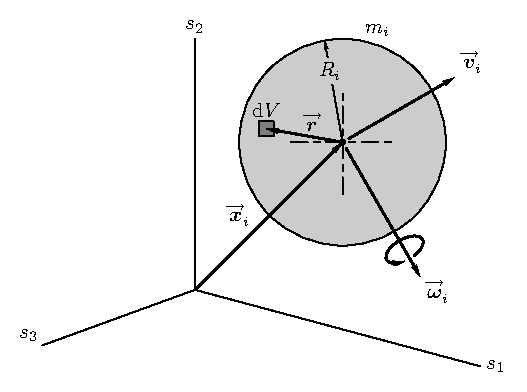
\includegraphics{figs/DEM-Def-Ball}
   \caption{Ball Element Parameters}
   \label{fig:BallDef}
\end{figure}


\subsection{Ball mass and inertia parameters}

Consider a volume element $\mathrm{d}V$ with respect to a static base $S$ of
an arbitrary solid body with  density $\rho$. The mass of the body is
obtained by integrating over the volume of the body,
\begin{equation}
    m = \int\limits_{\mathrm{body}} \rho\, \mathrm{d}V
    \label{eq:BMass-dif}
\end{equation}

In figure~\ref{fig:BallDef}, a ball with radius $R_{i}$ and uniform density
$\rho_i$ is depicted. The mass of the ball is after integration of
equation~\eqref{eq:BMass-dif}
\begin{equation}
    m_i = \tfrac{4}{3} \pi \rho_i\, R_i^3 .
    \label{eq:BMass}
\end{equation}


%----------------------------------------------------------------------------
\endinput

%\include{contents/App-2}
%\include{contents/App-3}

%==== Bibliography acro's & Index ===================================
\backmatter

\bibliography{backmatter/PHD}

\end{document}
